\section{Blockchain}
\subsection{Basic information}
The platform uses Ethereum blockchain that represents a single decentralized virtual machine (EVM). The desired system logic can be implemented using smart contracts.

\begin{note}[QUOTE]
A contract is a collection of code (its functions) and data (its state) that resides at a specific address on the Ethereum blockchain.

\hfill --- \href{https://solidity.readthedocs.io/en/develop/introduction-to-smart-contracts.html}{Introduction to Smart Contracts (Solidity manual)}
\end{note}




Thus, smart contracts are able to store data. For the data in the blockchain the abstract type system described above is still valid (but with some restrictions).



\subsection{A subsystem for working with the Blockchain}

\begin{note}
  Attention: implementation details could be different depending on the platform used. The description below is relevant for PC platform.
\end{note}

To provide an access to the Blockchain, node software includes the full implementation of Ethereum Node providing access by means of `JSON-RPC 2.0`.

Secret keys are stored in the encrypted storage. A user is prompted to set password at first application launch.

\begin{note}
  Although it is technically feasible to use an existing account, it is recommended to create new one.*
\end{note}

The application interface allows to:
\begin{enumerate}
\item Create new account
\item Import an existing account
\item Set up the backup of private storage
\end{enumerate}

\begin{note}
  Attention: It is recommended to set up the cloud backup since this will allow to keep an access to account even in the case when the computer will be physically unavailable.
\end{note}

\begin{note} \it
Software allows getting access to Ethereum node command line. This function is primarily intended for debugging. It is not recommended to use a command line if you do not understand its purposes.
\end{note}

\subsection{Internal tokens}
Economical interactions within the system are provided using internal ZNA tokens. They represent valid Ethereum tokens and can be bought and sold at exchange houses.

\subsection{Account concept}
\textbf{Account} in the platform allows user to interact with the system by playing several roles concurrently. Each role in account corresponds to separate smart contract in the blockchain.


\begin{figure}[H] \centering
  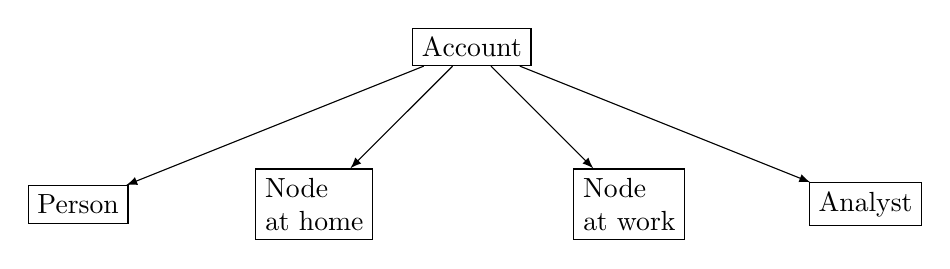
\begin{tikzpicture}
    \draw ( 0,  0) node [draw] (A) {Account}
          (-2, -2) node [draw, align=left] (N1) {Node\\ at home}
          ( 2, -2) node [draw, align=left] (N2) {Node\\ at work}
          (-5, -2) node [draw] (P) {Person}
          ( 5, -2) node [draw] (S) {Analyst}
    (A) edge [-latex] (N1)
        edge [-latex] (P)
        edge [-latex] (S)
        edge [-latex] (N2);
  \end{tikzpicture}

  \caption{The account of a user who has provided his or her genome (Person role) to the platform, who works as a bioinformatician and supports two computational nodes located at home and at work.}
\end{figure}

%\subsection{Participant role concept (draft)}

\textbf{Role} --- is a characteristic of the system participant regarding the specific type of interactions in which he or she takes part. Each participant may play several roles simultaneously.

%Role concept includes the following interrelated aspects:

%+ Requirements to the participant
%+ Available possibilities for interactions with the system
%+
%+

\begin{note}
  А separate subsystem is responsible for the role distribution.
\end{note}




%\subsection{Storing the data of abstract type in the blockchain}
%Let us say that smart contract contains the data of type `T` if there exists a natural way to represent these data as smart contract variables’ values, and the inverse transformation is also possible.

%-----

%For example, the following contract (taken from Solidity manual) implements the simple data storage:

%```js
%contract SimpleStorage {
%    uint storedData1;
%    uint storedData2;
%
%
%    function set(uint x1, uint x2) {
%        storedData1 = x1;
%        storedData2 = x2;
%    }
%
%    function get() constant returns (uint, uint) {
%        return (storedData1, storedData2);
%    }
%}
%```

%According to the last definition, this contract implements a pair of two elements of `uint` type:

%      data :: Tuple<uint, uint>

%Let us note that we can say that this contract implements a list consisting of two elements:

%      data :: List<2, uint>

%Less trivial example of data type implementation that enables its storing using the given smart contract is as follows:

%      data :: Record { storedData1 :: uint; storedData1 :: uint; };

%> This is not surprising: the same data could be represented in different ways even within main type system. It is also not surprising that there exists a number of ways to build a representation of `T` data type in a form of a smart contract. Inter alia, there are meaningless, yet formally valid, ways to do this.

%**This is why the building of data type representation in the blockchain should be directed by common sense and system logic.**
